\documentclass{ltjsbook}
\usepackage{docmute} 
\usepackage{../../myStyle} 

\begin{document}
\chapter{数値データの種類}
\label{m02_Numbers}
さて前回は，科学としての心理学なので，数量的なデータを扱って研究が進められる，という話をしました。今回は，何をどのようにデータにするか，データの種類と言った点についてお話しします。
\section{データと変数}
心理学では目に見えないものを研究対象とするため，心を持つと考えられる主体にたいして刺激を与え，その反応を見て「こうすれば(刺激)$\to$心のせいで$\to$こうなる(反応)」という因果を説明するためのモデルとして研究するのだ，ということでした。ここで刺激と反応は，研究対象である「心」の外にあって，観測できるものです。これをデータにしていきます。

図\ref{fig::03_01}は心理学研究の流れを説明したものです。ここで述べている「刺激と反応からデータを作る」というところは\keytermL{心理測定法}{しんりそくていほう}と呼ばれます。何をどのようにデータにするか，ということを考えるところであり，それぞれの心理学領域によって様々なバリエーションがあります。神経生理のような領域での研究であれば，データは計測機から得られる電気反応の強さ，間隔などになるでしょうし，認知・知覚・学習心理学のような領域であれば，たとえば被験者のキー反応の早さなどをPCで計測してデータとするでしょう。社会・学習・臨床心理学のような応用的領域であれば，被験者の発話，調査票への回答パターンなどがデータになるでしょう。いずれの領域でデータを取るにしても，ここで重要なのはそのデータの\keyterm{信頼性}{しんらいせい}{reliability}と\keyterm{妥当性}{だとうせい}{validity}です\footnote{詳しくは第\ref{m06_ctt}講で触れます。}。

\begin{figure}[ht]
	\centering
	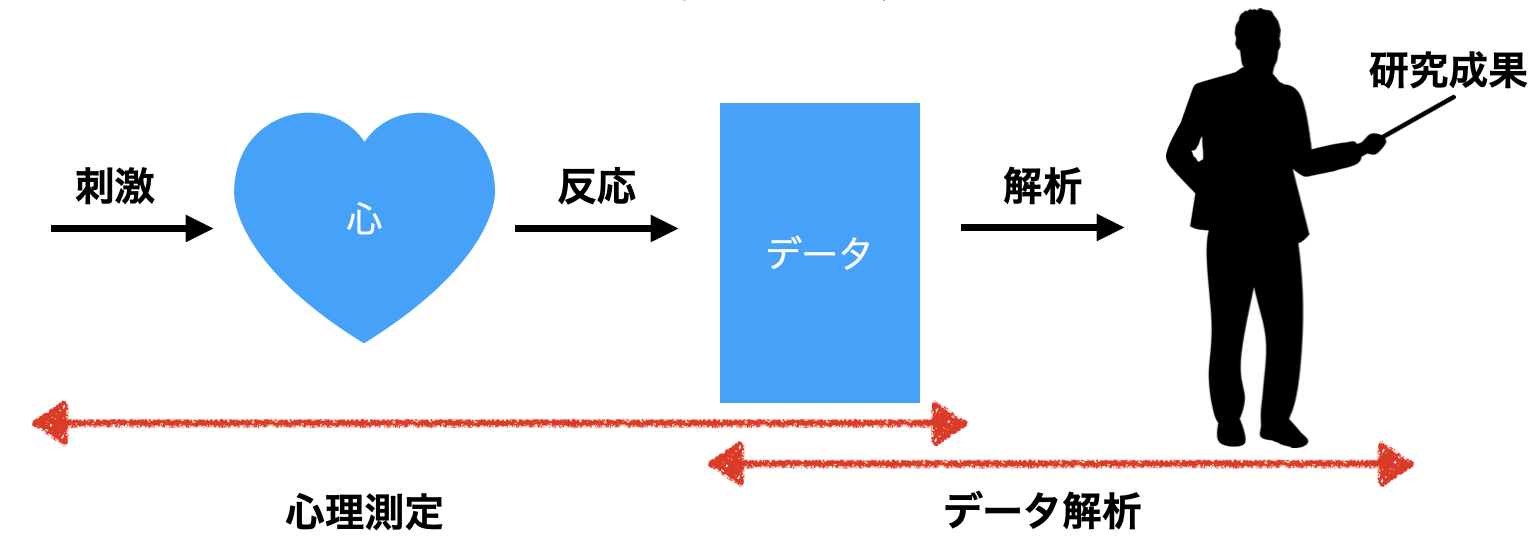
\includegraphics[keepaspectratio,width=12cm]{../images/02_Numbers/slide03_01.png}
	\caption{心理学研究のプロセス}
	\label{fig::03_01}
\end{figure}

それに対して，この講義でとくに重点的に議論するのは後半のデータ解析のところになります。つまりデータが得られた後で，それをどのように分析していくか，という点です。これについては次回も言及しますが\footnote{$\to$セクション\ref{reproducibility},Pp.\pageref{reproducibility}}，\keyterm{客観性}{きゃっかんせい}{objectivity}や\keyterm{再現性}{さいげんせい}{reproducibility}が重要になってきます。同じデータであれば誰でも同じ結果に到達できる，ということが重要ですし，言い方を変えると数学的に正誤の判断がついてしまう領域でもありますので，正しく理解し利用できるように学んでいきましょう。

\begin{figure}[ht]
	\centering
	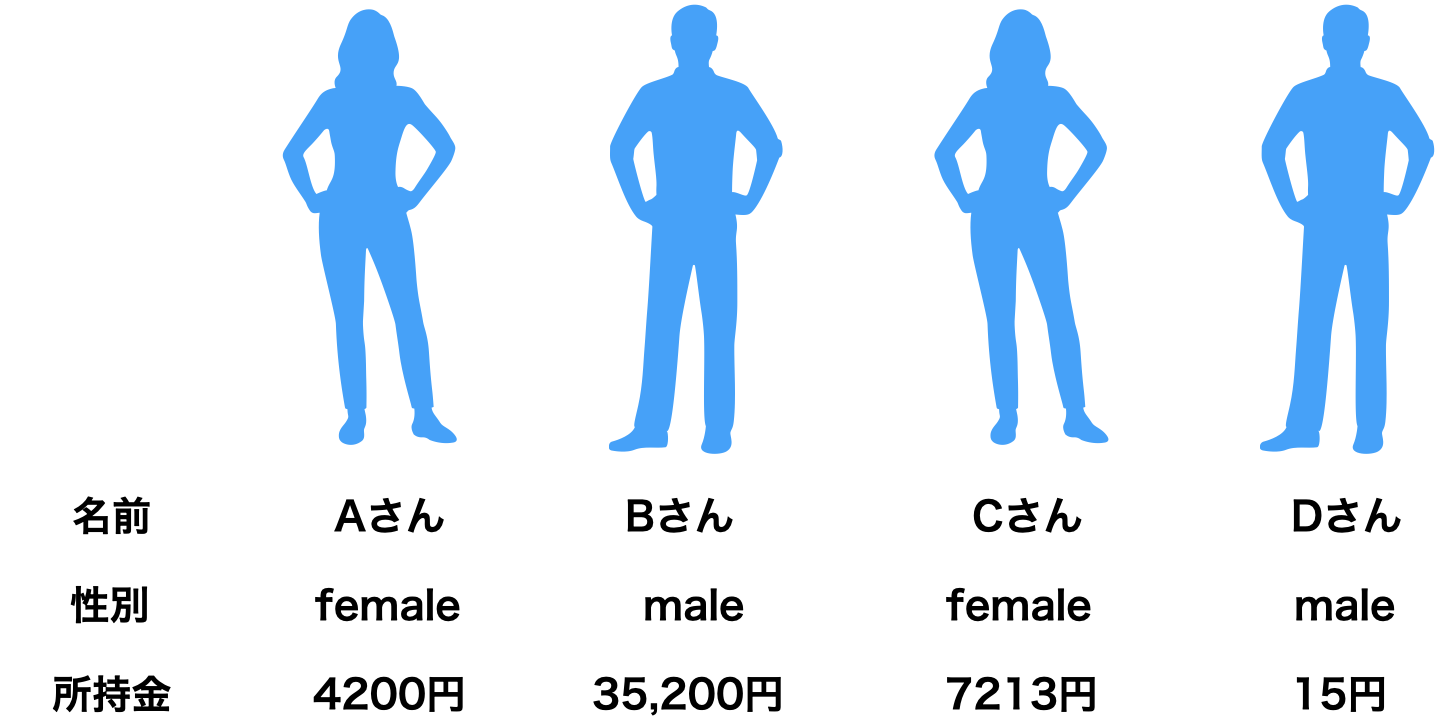
\includegraphics[keepaspectratio,width=12cm]{../images/02_Numbers/slide03_02.png}
	\caption{データって何?}
	\label{fig::03_02}
\end{figure}

さてこれからデータを分析していく話をするのですが，改めてデータとは何でしょうか。図\ref{fig::03_02}を見てください。ここには4人の研究対象者がいて，色々な情報を集めてみました。この中でデータとはいったい何を表すでしょうか。所持金は数字ですので，これだけがデータだ，と思ったら大間違いです。実は名前や性別もデータです。これらは全て数値化し，データとして扱えるものです。

少し用語の説明をしておきますと，名前，性別，所持金などは人によって\footnote{心理学でも研究対象が人でない場合がありますから，データの単位は他にも「個体」「ケース」などということがあります。英語のObservationを略してObs.と書かれることもあります。}変わる数字です。人によって変わる数字のことを\keyterm{変数}{へんすう}{variables}と言います。名前・性別・所持金は変数名であり，それがケースごとに「Aさん」「男性male」「15円」と変わるのです。ここで15円はともかく，名前や性別は数字じゃないぞ？ と思われるかもしれません。先にも述べたように，数字じゃないような実体であっても，これに数字を割り振るルールを決めて数字に置き換えていきます。このルールを決めることを\keyterm{尺度化}{しゃくどか}{scaling}と言います。

\begin{figure}[ht]
	\centering
	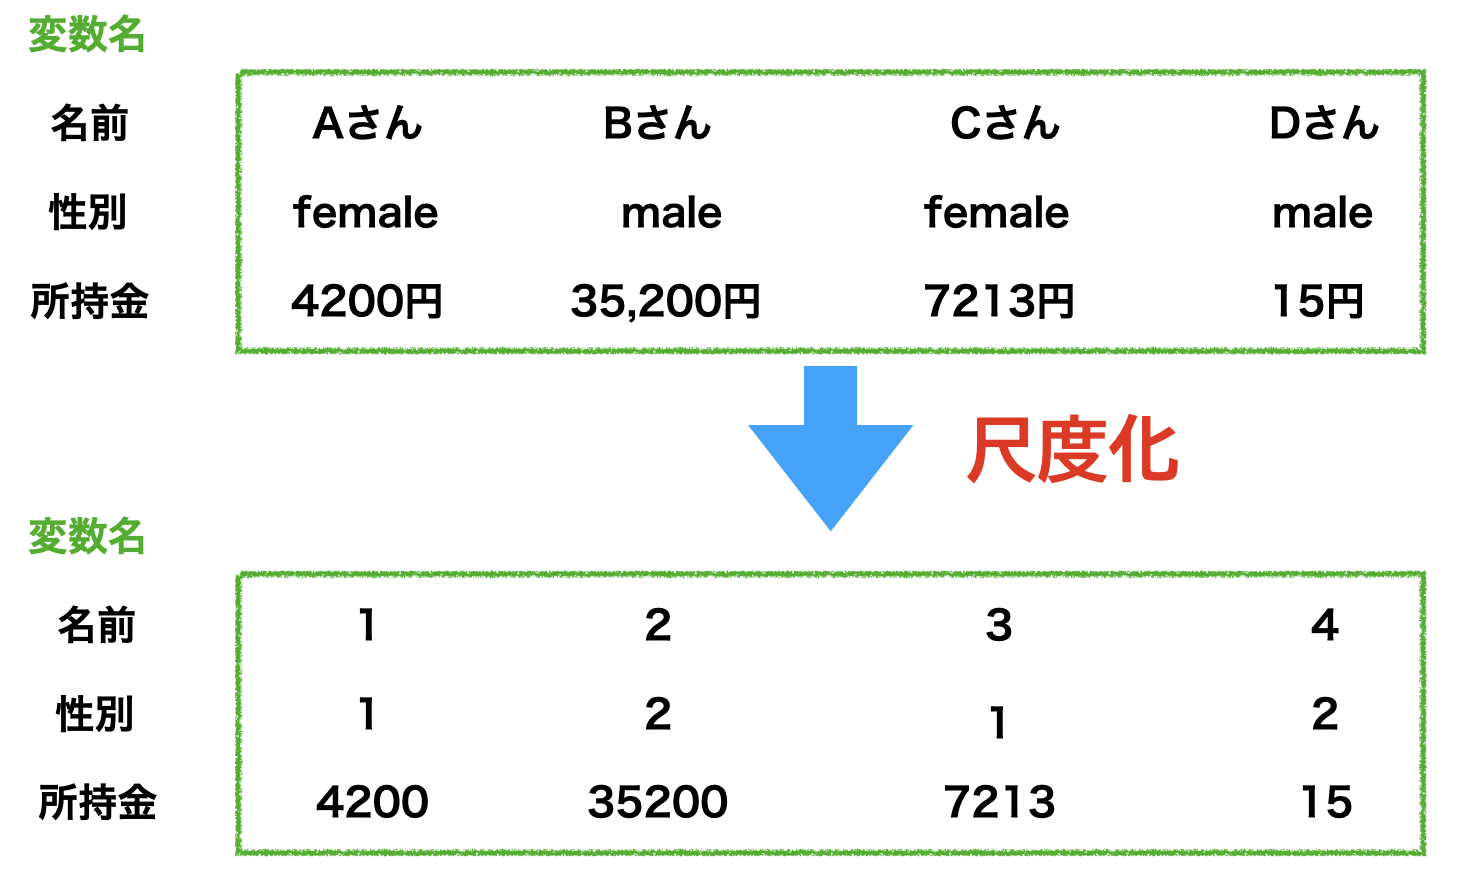
\includegraphics[keepaspectratio,width=12cm]{../images/02_Numbers/slide03_03.png}
	\caption{尺度化＝数値に置き換える}
	\label{fig::03_03}
\end{figure}

図\ref{fig::03_03}に数値化した例を挙げました。上の段にあるのが本来の情報であり，数値化されたのが下の段にあります。下の段は全て数字になっていますね。どこがどう変わっているのか，よく見ておきましょう。実際の統計的な分析をするときは電子計算機を使いますが，電子計算機にデータを与えるときは下の段にあるように数字だけにするのだ，と理解してください\footnote{ExcelやNumbersなどの表計算ソフトでは，その枠の中に日本語を書き込むことができます。しかし統計ソフトで扱う場合は，機械が内部では下段のような数字に置き換えているのだと思っておいてください。電子計算機の中では日本語も0/1の数列にすぎませんが。}。

こうしてみていても，数字には2種類あることがわかります。まず所持金を見てください。これは最初から数字でしたので，そのまま数字として扱っていきます\footnote{単位の「円」という文字は取れています。表計算ソフトに入力するときはこのように，数字以外のものは削ぎ落とすようにしてください。文字が入っていると数字として計算できないからです。ましてや2バイト文字なんて!}。このように本来の数字としての意味を持っているものは\keyterm{量的変数}{りょうてきへんすう}{numeric variable}と呼ばれます。一方で，性別は「女性female」を1に，「男性male」を2に置き換えています。名前に至っては，「Aさん」を1に，「Bさん」を2に，「Cさん」を3に，「Dさん」を4に置き換えています。これらの数字は人や性質を分類するためのものであって，数字に大小関係など量的な違いを表すものではありません。いわば質的な違いを表すための数字で，こうした変数は\keyterm{質的変数}{しつてきへんすう}{categorical variable}と呼ばれます。

このことからわかるように，「なんでも数字にして扱うが，数字には種類がある」ということに注意が必要です。なんでも数字にする，というと眉をひそめる人がいるかもしれません。心・気持ち・想いは数字にできない！と直観的に反論したくなる人もいるでしょう。しかし全くできないわけではないのです。というのも，言葉にできるのであればそれに適当な数字を割り振ることは可能だからです。数字が必ずしも大小関係を表すものばかりではないこともあるのですから。言葉にできるということは，質的に異なって分類できるということであり，それに数字のラベルを貼ることは可能です。一方，言葉にできない気持ちというのもあるでしょう。しかし，適切に言葉にできないのであれば，科学的な研究対象にはならないと言わざるを得ません。なぜなら「私だけが知りうる本当の気持ち」というのは，私秘性を徹底的に排除するという科学の基本姿勢に反するからです\footnote{言葉に言えないなんとも表現できない気持ちがない，と言ってるわけではないのです。科学的に研究できない，というだけで，私個人も色々な心の動きを経験しています。ただそれは私一人の思い出であって，研究対象にならないと言っているだけです。}\footnote{言葉にして数値化するというのは，心の一側面を捉えているにすぎない，という指摘も当然ありましょう。しかしだからと言って数字を使わない，というのはもったいないのです。また数字で表すことによって，どこまで表現できてどこまで表現できないか，というのも表現できたりします(正確には誤差の大きさを見積もる，という話で本講義の第\ref{m06_ctt}講ごろから触れていきます)。表現できるところはし尽くし，できないところについては黙って味わえば良いのであって，表現することを禁じるのは建設的な態度ではありません。}。

心理学の研究法の1つに，質問紙法というものがあります。複数の項目が並んでいて，それぞれに対して「当てはまる」「どちらかと言えば当てはまる」「どちらとも言えない」「どちらかと言えば当てはまらない」「全く当てはまらない」のどこかに丸をつけてください，という聞き方をするものが一般的です。たとえば「Q.この世の中では，努力がいつか報われるようになっていると思う」という問いに対して「自分の考え（気持ち，意見，態度）に最も近いところに丸をしてください」と言われ，ある人は「当てはまる」に丸を，別の人は「どちらかと言えば当てはまらない」に丸をつけたとしましょう。ここで「当てはまる」を5点，「どちらかと言えば当てはまらない」を3点，といった形で数値化すれば，大小関係は比較できるので量的変数として扱うことができます。この時ここで測りたいのは，「世界は公平だと思うか」というその人の心理的態度(信念)を測定していると考えられます。

このように回答のパターンを見ることで，目に見えない心の状態を数値化することもできます。見たいものは目に見えない心の状態ですが，測定して，点数をつけたりします。他にも，行動や振る舞いの記録など，知りたいことについて集められる情報は全てデータであり，分析対象になります。

\section{変数の分類}
\label{chap3sec2}
変数は，文脈や用途によって色々な分類がなされます。先ほど量的変数，質的変数という分類をしましたが，これは数値データの特徴による分類でした。他にも「潜在変数/観測変数」という違いや「原因変数/結果変数」といった違いを表すことがあります。ここではこの2つについて説明していきましょう。
\subsection{潜在変数と観測変数}
先ほど，個々人の考えや気持ちの強弱をその当てはまりの程度に置き換え，言葉の強弱から大小関係をもった数字で表す方法について説明しました(図\ref{fig::03_04})。言葉を点数に変える数字のルールを決めることを尺度化というのでしたね。どうして「どちらとも言えない」が3になるのか，ということについてはしっかりした理論が背後にありますがそれはおいおい説明していくことにして，話を先に進めます。

心理学の場合，ある心の状態(たとえば抑うつ状態にあるとか，性格特性がどれぐらいあるとか)を数値化するのに，複数の質問項目の合計得点を利用することがあります。このように，目に見えているデータを加工して，目に見えない変数の代わりにすることがあります。たとえばテストの正答数から合計得点を計算し，成績をつけるということもあるでしょう。これは正答率が学力を反映しているという前提の下での尺度化です。学力も心と同じで，目に見えない想定される心的状態のひとつですね。

\begin{figure}[ht]
	\centering
	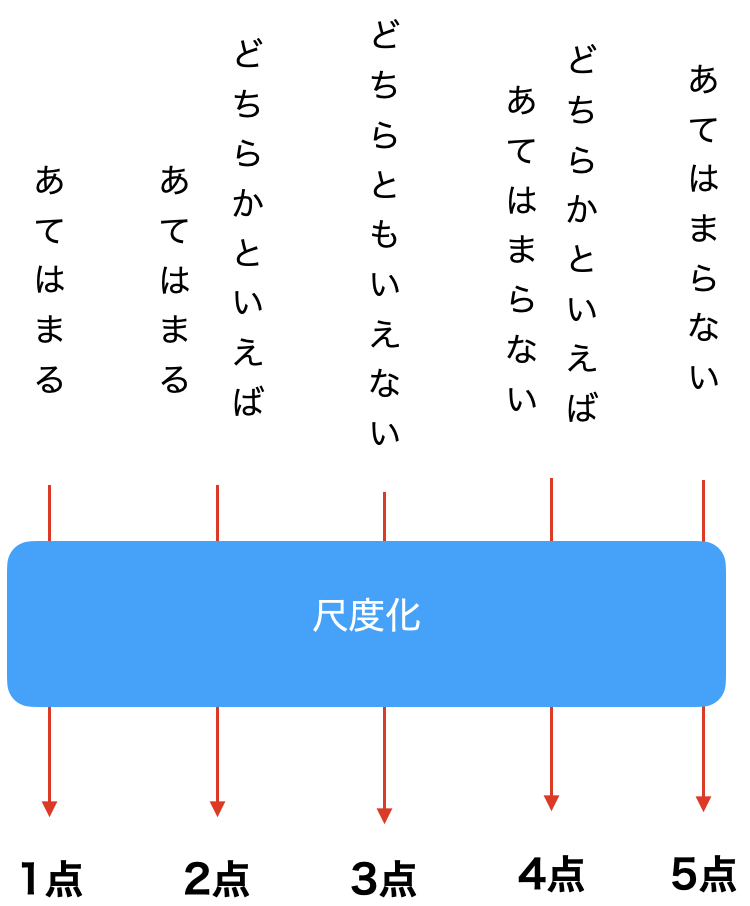
\includegraphics[keepaspectratio,width=6cm]{../images/02_Numbers/slide03_04.png}
	\caption{尺度化による数字への置き換え}
	\label{fig::03_04}
\end{figure}

心理学では人間の振る舞いの背後に心というモデルを仮定し，それをデータという目に見える数値をつかって表現するものです。目に見えるように尺度化されたデータのことを\keyterm{観測変数}{かんそくへんすう}{observed variables}とか\keyterm{アウトカム変数}{あうとかむへんすう}{outcome variables}と言います。これに対して，観測変数から算出してモデルの状態を表現した変数のことを\keyterm{潜在変数}{せんざいへんすう}{latent variables}と言います。心理学では測定を数理的にモデル化し，モデル上想定される変数をモデルの中で加工したりすることがあります。潜在変数は具体的な数字に顕現化していませんが，抽象的なモデルのままで計算を進めたりできるのです。具体的には測定モデルについての説明が必要になりますが，ここでは観測変数だけでないものも扱えるのだ，ということを知っておいていただければ十分です。

\subsection{原因変数と結果変数}
変数をその研究の用途から分類することもあります。たとえば次のような研究仮説を考えてみてください。
\begin{enumerate}
	\item 家族療法を一定期間受けた拒食症の若年女性の，治療前と治療後の体重を記録した。家族療法が有効な治療法であったと言えるか?
	\item ラットのある群には自由に食事を与えられ，もう一方には非常に低カロリーな生活をさせた。食事スタイルは寿命にどのように影響するか?
\end{enumerate}
さてこれらのケースで，変数に当たるのはどこになるでしょうか。分析するときに必要な情報の単位が変数になりますので，注意深く読んで考えてみてください。

最初の例では，「治療前か治療後か」という違いが分析上必要ですので，この測定のタイミングが1つの変数になります。もう1つはもちろん体重ですね。この体重が変わったかどうかが知りたいのですから。2つ目の例では，寿命の長さ(何日生きるか)が変数だというのはすぐに気づくと思いますが，もう1つ，「ある群」と「もう一方」，つまり「自由に食事ができるか，低カロリーなものしか食べられないか」という違いも変数なのです。これらの情報をデータとして記録しておかないと，体重や寿命の長さの数字だけ見せられても意味がないですね。

ここでの例はいずれも，複数の変数間関係を「原因」と「結果」に分けて検証するというものでした。
\begin{enumerate}
	\item 介入の前と後(原因)$\to$体重(結果)
	\item 食事カロリーの違い(原因)$\to$寿命(結果)
\end{enumerate}
「介入前のデータなのか，後のデータなのか」も``変化する''指標なので，変数として扱う，というのがポイントです。この例にあるように，研究仮説の観点から，原因としたい変数のことをとくに\keyterm{予測子}{よそくし}{predictor}，\keyterm{説明変数}{せつめいへんすう}{explanatory variable}，\keyterm{独立変数}{どくりつへんすう}{independent variable}\footnote{結果から独立している，という意味です。}などと呼びます。結果になる変数は\keyterm{被予測変数}{ひよそくへんすう}{predicted variable}，\keyterm{被説明変数}{ひせつめいへんすう}{explained variable}，\keyterm{従属変数}{じゅうぞくへんすう}{dependent variables}とも呼ばれます。

変数は数字で表されます。たとえば介入前を0，介入後を1というように，です。介入の前後を表す変数を$x$，結果としての体重を$y$と表すと，この研究は$y=f(x)$，つまり関数関係を明らかにすることであるとも言えます\footnote{$y=f(x)$のfはfunctionのfで，functionは関数とも機能とも訳されます。}。心理学が科学であること，科学であるということは数学的現象主義をとること，数値化によってモデルを検証できること，がこのように繋がっているのです。もちろん関数の形がどんなものなのかは，現象によって様々なものが考えられるでしょう。

ただし，データを使って一方の変数から他方の変数を予測する，というのは，研究者の「仮説」に過ぎないことに注意してください。本当のことがわからないので，一方を原因，他方を結果とおいて考えようというだけで，本当の因果の向きは逆かもしれないのです。その仮説が正しいかどうかは，予測が当たるかどうかで評価することが基本です。もっとも，人間の行動は複雑なので(あるいは測定が非常に難しいので)，なかなかうまくいくものではありませんが。

また因果関係は「原因」になるのが先にあり，「結果」が後に来るはずです。研究の中には，同時に取ることで得られるデータもあります。同時に取られた複数の変数間関係からは，変数同士の関係の強さを数値化できます(第\ref{m08_CorrelationCausation}講で詳しく説明しますが，相関係数と呼ばれます)。ただし，相関関係＝因果関係ではないことに注意が必要です。相関関係は相互に関係があることを示すだけで，どちらが原因でどちらが結果なのかは分かりません。因果関係は時間的な位置関係は明確です。それに加えて，原因変数の背後にさらなる原因変数があるかもしれませんし，原因変数と結果変数の間に共通する媒介変数があるかもしれません。確認されていないだけで，逆の因果関係があるかもしれません。このように，データや数字から表現できることは色々ありますが，それを解釈するのはあくまでも人間側の問題なのです。全く中立なデータやモデルというのはなく，常になんらかの仮定や前提，主張を含んだ表現であることを忘れないでください。


\section{尺度水準による分類}

変数には様々な名称があることを見てきましたが，今度は尺度化された数値に着目してみましょう。数字になってしまえば全部同じか，というと実はそうではありません。\citet{stevens1946}は数値が持つ情報とそれに伴う計算可能性の観点から，尺度を4つの水準に分類しています。それぞれ次のような名前がついています。
\begin{enumerate}
	\item \keyterm{名義尺度水準}{めいぎしゃくどすいじゅん}{nominal scale}
	\item \keyterm{順序尺度水準}{じゅんじょしゃくどすいじゅん}{ordinal scale}
	\item \keyterm{間隔尺度水準}{かんかくしゃくどすいじゅん}{interval scale}
	\item \keyterm{比率尺度水準}{ひりつしゃくどすいじゅん}{ratio scale}
\end{enumerate}

名義尺度水準が最も下のレベルで，比率尺度水準が最も上のレベルという階層性を持っています。上に上がるほど徐々に条件が強くなっていきます。逆に言えば，上の尺度水準に該当する変数をより下位の水準の変数として扱うことが可能です。このことについて詳しくは後ほど説明するとして，それぞれがどういう意味なのかを説明していきましょう。

\paragraph{名義尺度水準}
最も下位のレベルにある水準です。この水準にある数値は，数字ではありますが数字としての意味がないレベルです。単にラベルとして対象に数字を割り当てた，というだけのとき，その数字は\keytermL{名義尺度水準}{めいぎしゃくどすいじゅん}にある，と言います。この講のセクション\ref{chap3sec2},Pp.\pageref{chap3sec2}で，性別や名前に数字を割り当てたのを思い出してください。たとえば女性に1を，男性に2を割り当てたとします。この割り当てられた数字に，深い意味はないですね。別に男性が2でもいいし，女性に43543という数字を当てておいても良いわけです。数字だけ見ても，女性が男性の2倍あるとか，男性より少ない・小さいことを意味しているわけではありません。あるいはみなさんが持っている携帯電話の番号もこの尺度水準です。みなさんの数字はどれひとつとして同じではないですが，その数字に深い意味はないですね\footnote{語呂合わせがしやすいかどうか，というのはありますが。}。他にも学籍番号や，名前に割り当てられた数字(Aさんが1,Bさんが2など)に数字としての特徴はなく，ただの名前を簡略化したものに過ぎません。こういう数字のことを名義尺度水準にある数字，というわけです。

この水準の数字は，数字が大小関係や順序関係を表さないので，計算ができません。たとえば女性を1，男性を2と尺度化したデータを集めて平均値を出したら1.7でした，と言っても意味がないのです。1.7に該当する対象がないのですから。この尺度水準では\texttt{数字と対象が一対一対応していること}が重要なのであって，数字を計算して変化させても意味がありません。ではこの尺度水準の数字はなんの役にも立たないのか，と言われるとそんなことはありません。違う数字が割り振られていることから違う対象であることは分かりますので，分類するという性質は持っていますし，何よりどんな複雑な対象であっても名義尺度水準の数値は割り当てられるのです。その意味では，この後に出てくるどんな尺度水準よりも豊富な情報を含んでいる数値である，とも言えます。また，言葉にできなければ研究対象にできないという話をしましたが，言い換えると言葉にできるのであれば名義尺度水準の数値が割り当てられるということでもあります。

\paragraph{順序尺度水準}
名義尺度水準は数字としての意味を持たない，と言いました。これに順序関係，すなわち数字の大小に意味があるという条件が加われば，それは\keytermL{順序尺度水準}{じゅんじょしゃくどすいじゅん}の数字だということができます。たとえば好きな夕飯のメニューとして1番がカレー，2番がハンバーグだと答えた人がいたら，カレーの方がハンバーグよりも好まれている，価値が高い，優先されているという情報は得られるわけです。あるいは100m走での順位を表す数字だと，2と7を比べれば2位の人の方が速いんだな，ということがわかります。この程度の情報が含まれている数字のことを，順序尺度水準であると言います。ただこの水準の数字は大小関係を表すだけで，それ以外のことはわかりません。たとえば着順の話でも，1，2，3の順で優劣がついていることはわかるのですが，「1位がぶっちぎりだった」「団子レースだった」といった違いは表現できていないわけです。図\ref{fig::03_05}を見てもらうとわかるように，データとしては1,2,3という数字だけですから，上図のような状態でも下図のような状態でもデータとしては1,2,3,4であり，上図の2と下図の2を区別できません。まだ少し不便ですね。このように大小しかわからないので，計算にもまだ使えません。1位と2位を足して3位になるはずもないですし(そもそも逆転してますが)，2位と3位を足して1位と勝負できるかということもわからないのです。もちろんかけたり割ったりもできませんので，この水準の数字は四則演算ができません。

\begin{figure}[ht]
	\centering
	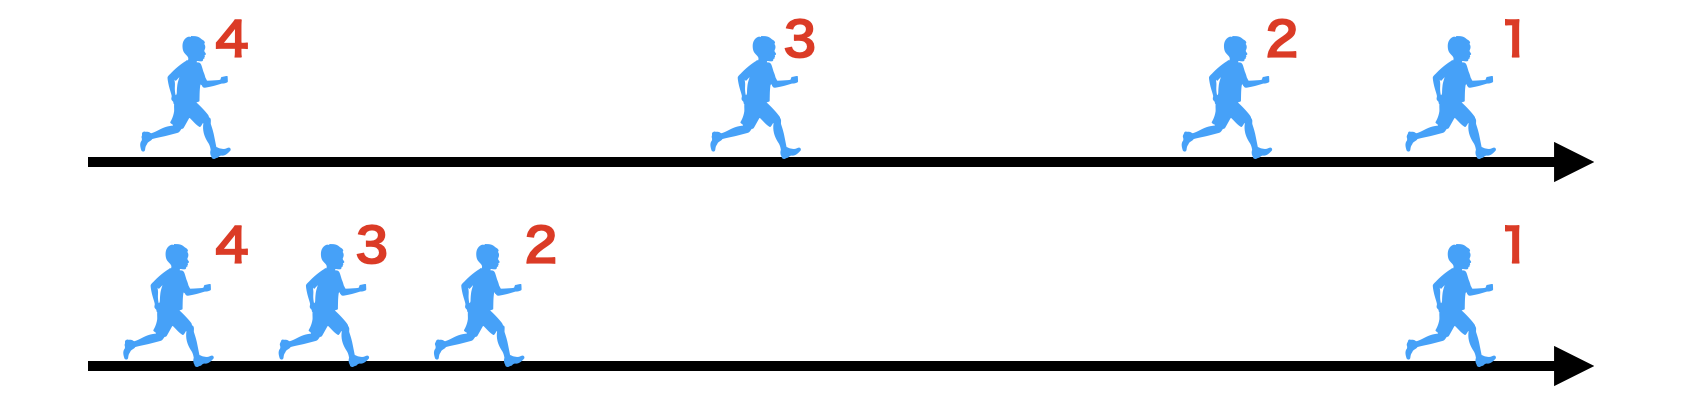
\includegraphics[keepaspectratio,width=12cm]{../images/02_Numbers/slide03_05.png}
	\caption{順序では程度がわからない}
	\label{fig::03_05}
\end{figure}

とはいえ，この水準の数字は，心理測定において最もおもしろいところであると言えるかもしれません。みなさんご自身の心の状態を数字で表すとして，さてその数字はどの水準にあるのでしょうか。たとえば「カレーはハンバーグの100倍美味しい！」と思っていても，本当に100倍という計算ができるような精度の高い数字でしょうか？ せいぜい優先順位の違いぐらいで，カレーを5点，ハンバーグを4点，餃子を3点・・・と採点していっても，カレーとハンバーグの違いが，ハンバーグと餃子との差と同程度であるとまでは言えないのではないでしょうか。ことほど左様に，心理学的な評価水準はせいぜい順序尺度水準であって，差や比の計算をするには，さらに上の尺度水準でなければなりません\footnote{しかし実際には，評定値を間隔尺度水準の値を持っているとみなして分析をすることが多くあります。これには\keytermL{心理測定法}{しんりそくていほう}の理論と歴史的な経緯があって，その両方を踏まえた上でことであればそのような「みなし」も正当化されます。残念なことに，それらを踏まえずして仮定が満たされていないのに勝手に間隔尺度水準だと思って使っている誤用例も数多くあるのですが。}。

\paragraph{間隔尺度水準}
\keytermL{間隔尺度水準}{かんかくしゃくどすいじゅん}は，順序尺度水準に加えて数値と数値の間隔が等しいという条件を追加したものです。順序尺度水準は1と2の差が2と3の差と違っても構わないのですが，間隔尺度水準ではこれがあっている必要があります。
代表的な例として，摂氏(温度)があげられます。これは水が氷になる氷点を0，水が水蒸気になる沸点を100とし，その間隔を百等分した目盛りによって温度を表現するものです\footnote{セルシウスさんが考えた方法なのでセ氏といいます。ちなみに定義上このようになっているのであって，「水ってちょうど0度で氷になって，ちょうど100度で水蒸気になるの，奇跡じゃない?」というのは悪いジョークです。}。このようにそもそも等間隔になるようにつけた目盛りですから，当然間隔尺度水準の数値であると言えます。この時，10℃と20℃の差は20℃と30℃の差と等しいといえますから，これは$20-10=30-20$と引き算の計算ができるレベルになっているわけです。

しかし，10℃は20℃の2倍の熱量を持っている，とは言えません。というのも，この数字は0℃に意味がないからです。言い換えると，0℃は温度が「ない」ことを意味するのではなく，0℃という温度が「ある」状態です。0がスタート地点ではないのです。スタート地点は任意に決められますから，たとえば
氷点を100，沸点を200とした新しい温度体系Xを作ったとします。このとき10℃は110Xで，20℃は120Xですから，$20/10\neq 120/110$ですね。同じ状態を表している数字なのに計算が合わないのはおかしいわけです。このような割り算の計算をするためには，さらにもうひとつ条件を追加する必要があります。

\paragraph{比率尺度水準}
\keytermL{比率尺度水準}{ひりつしゃくどすいじゅん}は，間隔尺度水準に加えて絶対0点を定めたものです。絶対0点とは，0が「ない」ことを意味する点のことです。たとえば0cmは長さがないのです。0kgは重さがないし，0秒は時間が経ってない，です。このように原点0が決まっている数値体系になって初めて，加減乗除の四則演算全てに対応できます。例に挙げたように，物理的な測定単位はほとんど比率尺度水準ですから，精緻に測定すればかなり細かい予測値まで計算できるのですね。これに対して心理学のデータで主観的につけられる評定値はせいぜいが順序尺度水準なので，物理学のようになかなかうまくいかないところもあるというのが実際です。心理学のデータでも客観的で比率尺度水準の数字を扱えるものもありますし(反応時間を指標とする，など)，主観的な評定値でも工夫して間隔尺度水準以上の数値にすることもあります。

みなさんが今後，どのようなデータをとって分析するようになるかは進む専門領域によって変わると思いますが，どの数字がどの尺度水準にあるのかについて，常に注意しておいてください。というのも，名義尺度水準や順序尺度水準では加減乗除の計算ができないので，分析の方法にも限界があるからです。これら尺度水準の違いは，統計ソフトウェアで分析するときもどの尺度水準にあるのか指定する必要があります。指定がなく全て計算可能な数値であると機械が誤認すると，頓珍漢な分析をしてしまうことになります。表\ref{tab::03_01}に\citet{stevens1946}によるまとめを引用しましたので確認しておいてください\footnote{\citet{stevens1946}の仕事をより正確に言うなら「測定対象全体に数値を与える適正な規則とは何か」を考えたのではなく，何らかの測定がなされた尺度がいくつかあれば，それらを相互に変換する規則が定められて，それが表にあるような4種類になるだろう，と言う考え方です。詳しくは\citet{吉野諒三2007}を参照してください。}。

\begin{table}[ht]
	\centering
	\caption{尺度水準のまとめ}
	\begin{tabular}{cccc}
		尺度水準                                       & 基本的な操作             & 数学的な群構造                                                              & 可能な統計量                                                               \\\hline\hline
		\begin{tabular}{c}名義\\Nominal\end{tabular}   & 同質性の判定             & \begin{tabular}{c} 置換群 \\ $x'=f(x)$\\$f(x)$は一対一対応  \end{tabular}   & \begin{tabular}{c}ケース数,\\最頻値,\\一致係数\end{tabular}                \\\hline
		\begin{tabular}{c}順序\\ Ordinal\end{tabular}  & 大小関係の判定           & \begin{tabular}{c} 同調群 \\  $x'=f(x)$\\$f(x)$は単調増加関数 \end{tabular} & \begin{tabular}{c}中央値, \\パーセンタイル\end{tabular}                    \\\hline
		\begin{tabular}{c}間隔\\ Interval\end{tabular} & 間隔や差分の等しさの判定 & \begin{tabular}{c} 一般線形群\\$x' = ax + b$ \end{tabular}                  & \begin{tabular}{c}平均値 ,\\ 標準偏差,\\  順序相関,\\積率相関\end{tabular} \\\hline
		\begin{tabular}{c}比率\\ Ratio\end{tabular}    & 比率の等しさの判定       & \begin{tabular}{c} 類似性群\\$x'=ax$ \end{tabular}                          & \begin{tabular}{c}変動係数 \end{tabular}                                   \\\hline
	\end{tabular}
	\label{tab::03_01}
\end{table}



統計処理の観点からは，間隔尺度水準と比率尺度水準はいずれも計算できるので量的データ，名義尺度水準と順序尺度水準は(計算できないので)質的なデータと2分割で済ませることもあります。他にも正の整数しか取らない離散的なデータをカウントデータと呼ぶこともあります。また，0と1の2つの値しか取らないデータを二値binaryデータと呼ぶこともあります。二値データは，0と1がそれぞれ男性と女性，正と誤，真と偽といったように様々な解釈ができますし，名義尺度水準でありながら数学的には量的データのように計算できることもあって，少し特別な位置付けにあるといえるでしょう。

\section{データの可視化}
\label{dataVisualization}
さて，ここまで変数の分類や数値の分類について語ってきました。こうした違いに注意しながら，これから分析を進めていくことになります。分析の第一歩は\keyterm{可視化}{かしか}{visualization}です。\textbf{データは図にする}のが基本中の基本です。みなさんもこれから演習や研究の一環で様々なデータを取ると思いますが，\textbf{データは図にする}のが基本です。これを忘れないでください。大事なことなので2度いいました。また，これから分析の話が28講分ありますが，\textbf{データは図にする}ということの重要性を強調するのは今回限りになります。しかし本当はこの重要性を常々言い続けていたいぐらいなのです。分析が進み，様々な知識や技術をみなさんに伝えていく中で，相対的に\textbf{データは図にする}ということの重要性が下がっていくように感じられるかもしれませんが，それは間違いです。取ったデータは最初に必ず図にしてください。様々な角度から図にしてください。なんならまだ取っていないデータであっても，このような図が得られるはずだとか，このような図を得るためのデータが欲しいと考えるようになってください。可視化することでわかりやすくなります。気づかなかったことが目で見てわかるようなヒントが得られます。一枚の図から様々な情報を読み取ることができるようになります。それほど可視化は重要なのです。

逆に言えば，可視化しなければ数字だけの羅列になります。数字の羅列が好きだという人は少ないと思いますが，そういう人はかえって数字を過大評価し，嫌いな数字を見つめているのが嫌だからでしょうか？ 1つの数字だけ見て大体わかったような気になってしまうのです。それではデータの本質がわかりません。データサイエンスの領域は今後ますますニーズが高まる領域ですが，優秀なデータサイエンティストは手に入ったデータを可視化して眺める時間をたっぷりとるものです\footnote{とある分析屋さんは，データの可視化に1週間ぐらいかけて，何百枚というグラフを眺めながらどうやって分析するかの筋道を見つけ出すと言ってました。}。とりあえず(決まり切った)分析をして指標を算出するというのは，時間の無駄になることも少なくないので，このことをしっかり意識しておいて欲しいと思います。

得られたデータは基本的に可視化しなければならず，そこから分析は始まっていると言えます。またそこにおいても再現性が重要です。ボタンをぽちぽち適当に押していたら出来上がった図，というのは再現性に乏しくチェックすることもできないので，図を書くためにも図を書くルールが必要です。表計算ソフトウェア\footnote{MicrosoftのExcel, Apple のNumbers, フリーソフトウェアのLibreOfficeにあるCalcsなどがそうです。}は簡単に図を作ってくれますが，GUI操作になりますので，統計環境のRやコンピュータ言語のPythonなどではCUI，すなわちコマンド(スクリプト，プログラム)で図を書きます\footnote{ひとつ1つの命令文のことをコマンド，複数のコマンドからなる一連の命令文をスクリプト，スクリプトがたくさん集まったものをプログラム，といいます。コマンドやスクリプトを描くことをプログラミングと呼ぶこともあります。}。図を書くのもプログラミングなのです。

この講義では統計環境Rを使っていきますが，Rには図を書くためのパッケージとして\texttt{ggplot2}\citep{ggplot2}というものがあります\footnote{統計環境Rについては第\ref{m03_introR}講で触れます。ひとまずは統計分析用のプログラミング言語だと理解しておいてください。またパッケージとは，特定の分析や機能に特化し追加で導入できる関数群のことです。}。可視化の文法については，心理学業界ではまだ広く浸透した概念とは言い難いのですが，見た目の美しさのみならず，論理的な美しさや再現可能性の観点から考えて極めて重要ですのでここで概略だけ説明しておきます。，まずはどのようなグラフが描けるのか，いくつか例をあげてみましょう。

\begin{figure}[ht]
	\centering
	\includegraphics[keepaspectratio,width=12cm]{../images/02_Numbers/ggplot_sample_01.png}
	\caption{ggplot2による出力例1}
	\label{fig::03_06}
\end{figure}

\begin{figure}[ht]
	\centering
	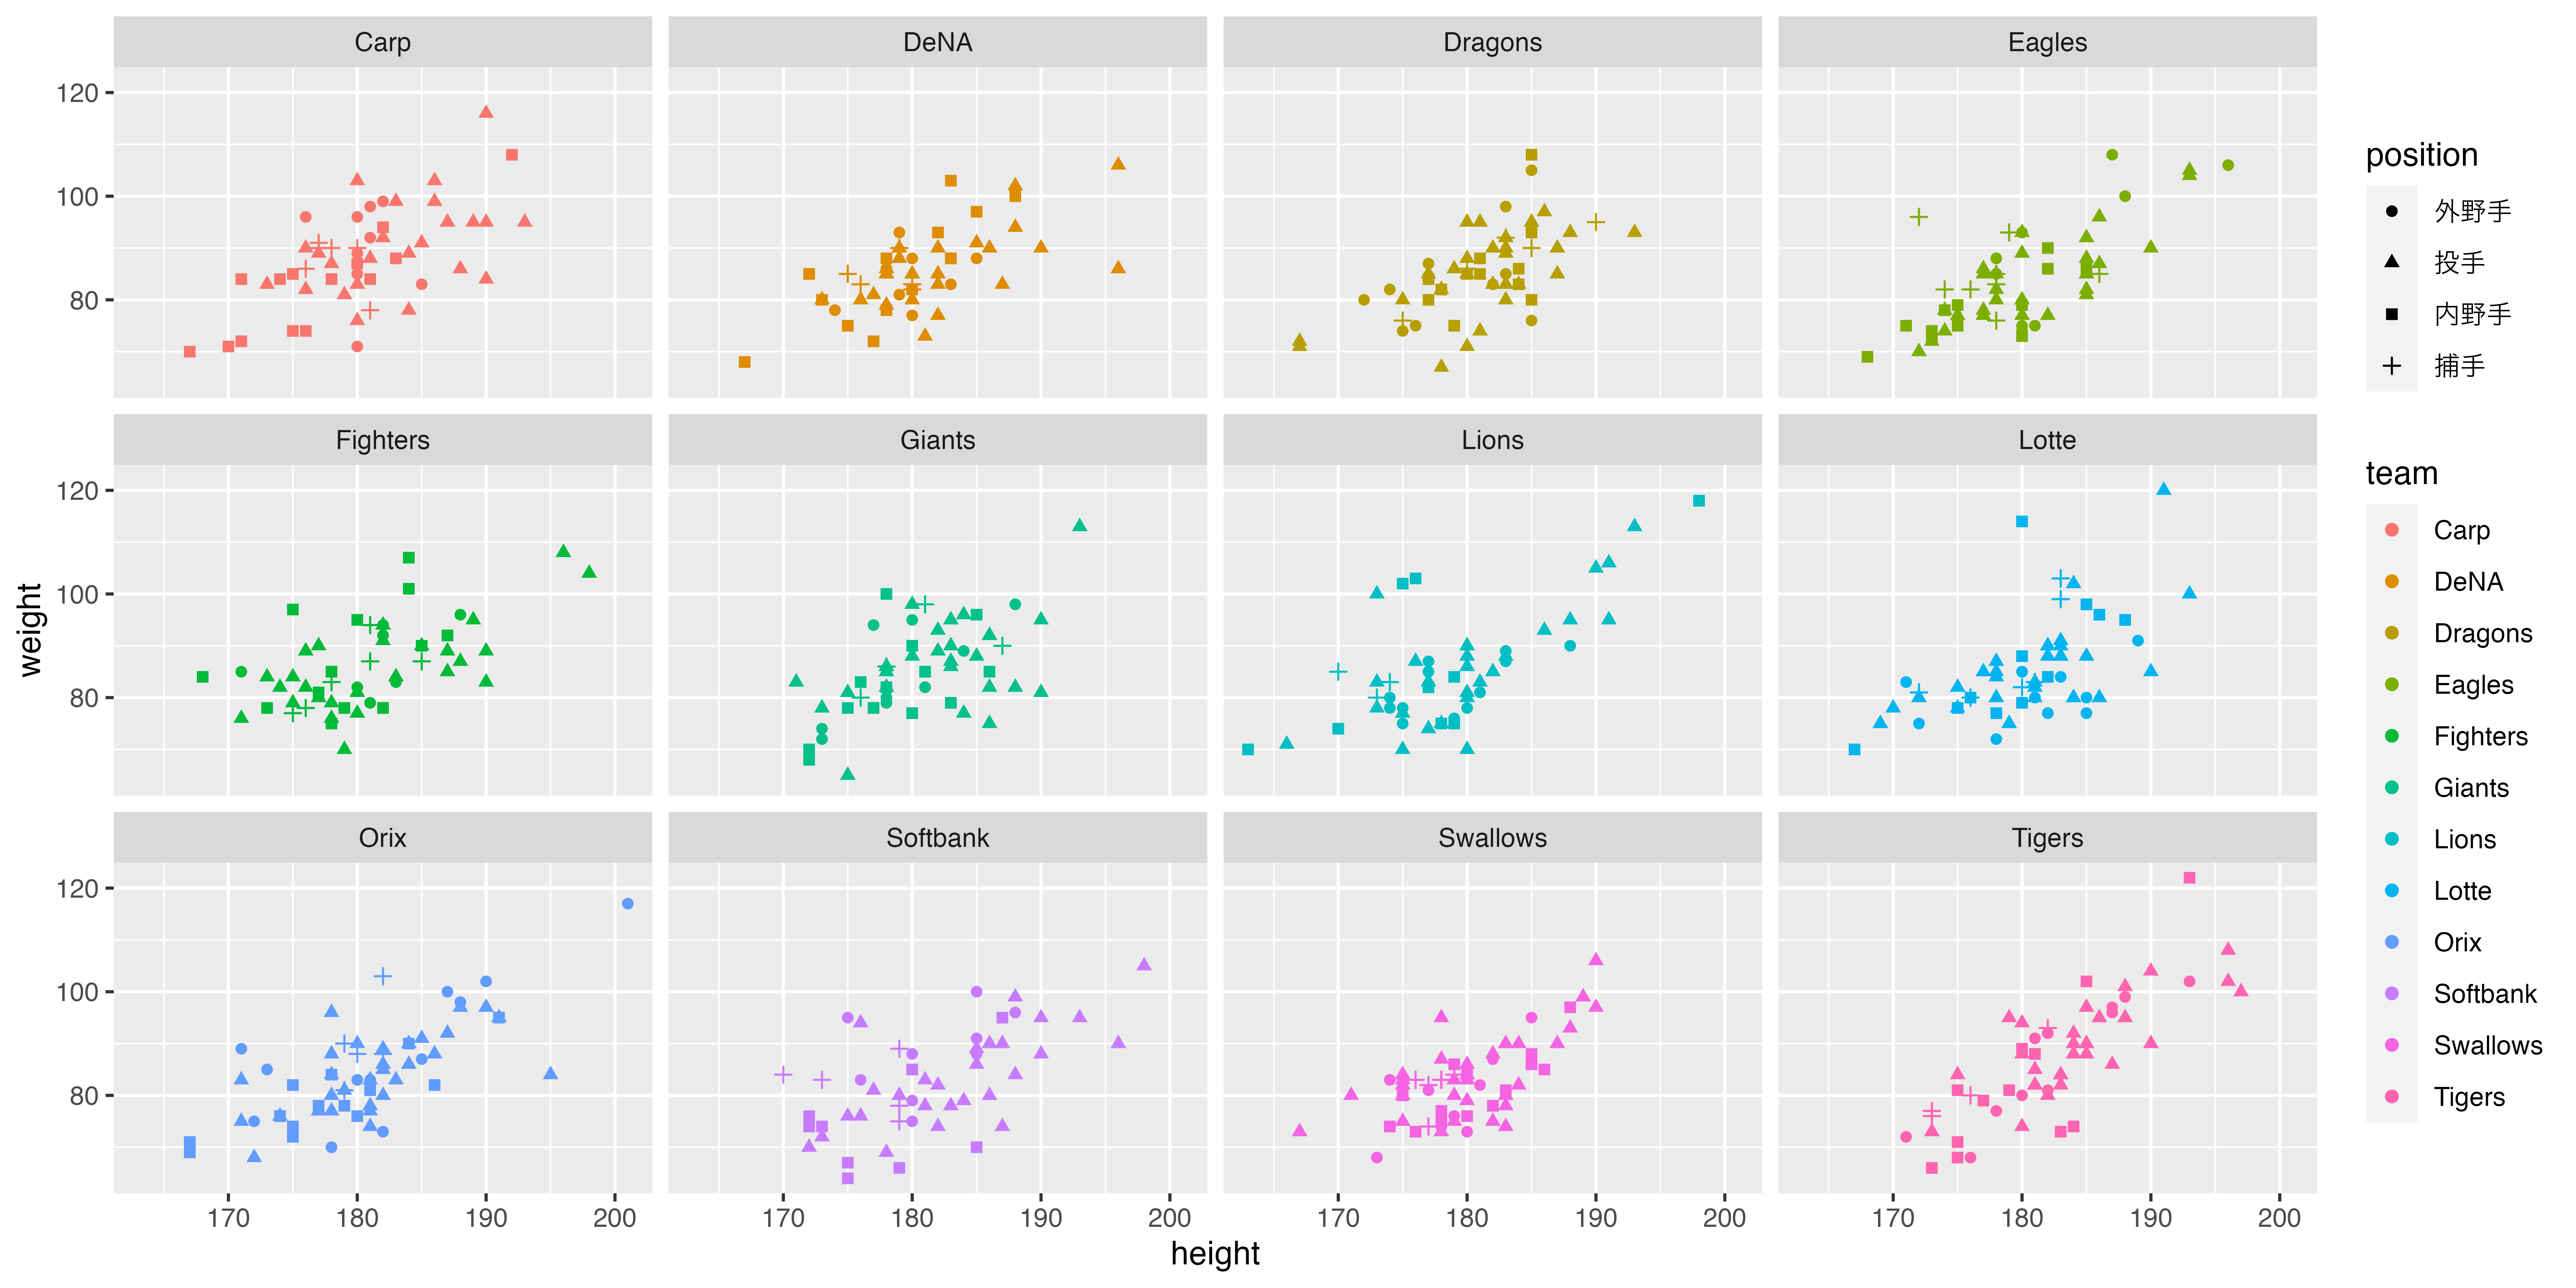
\includegraphics[keepaspectratio,width=12cm]{../images/02_Numbers/ggplot_sample_02.png}
	\caption{ggplot2による出力例2}
	\label{fig::03_07}
\end{figure}
\begin{figure}[ht]
	\centering
	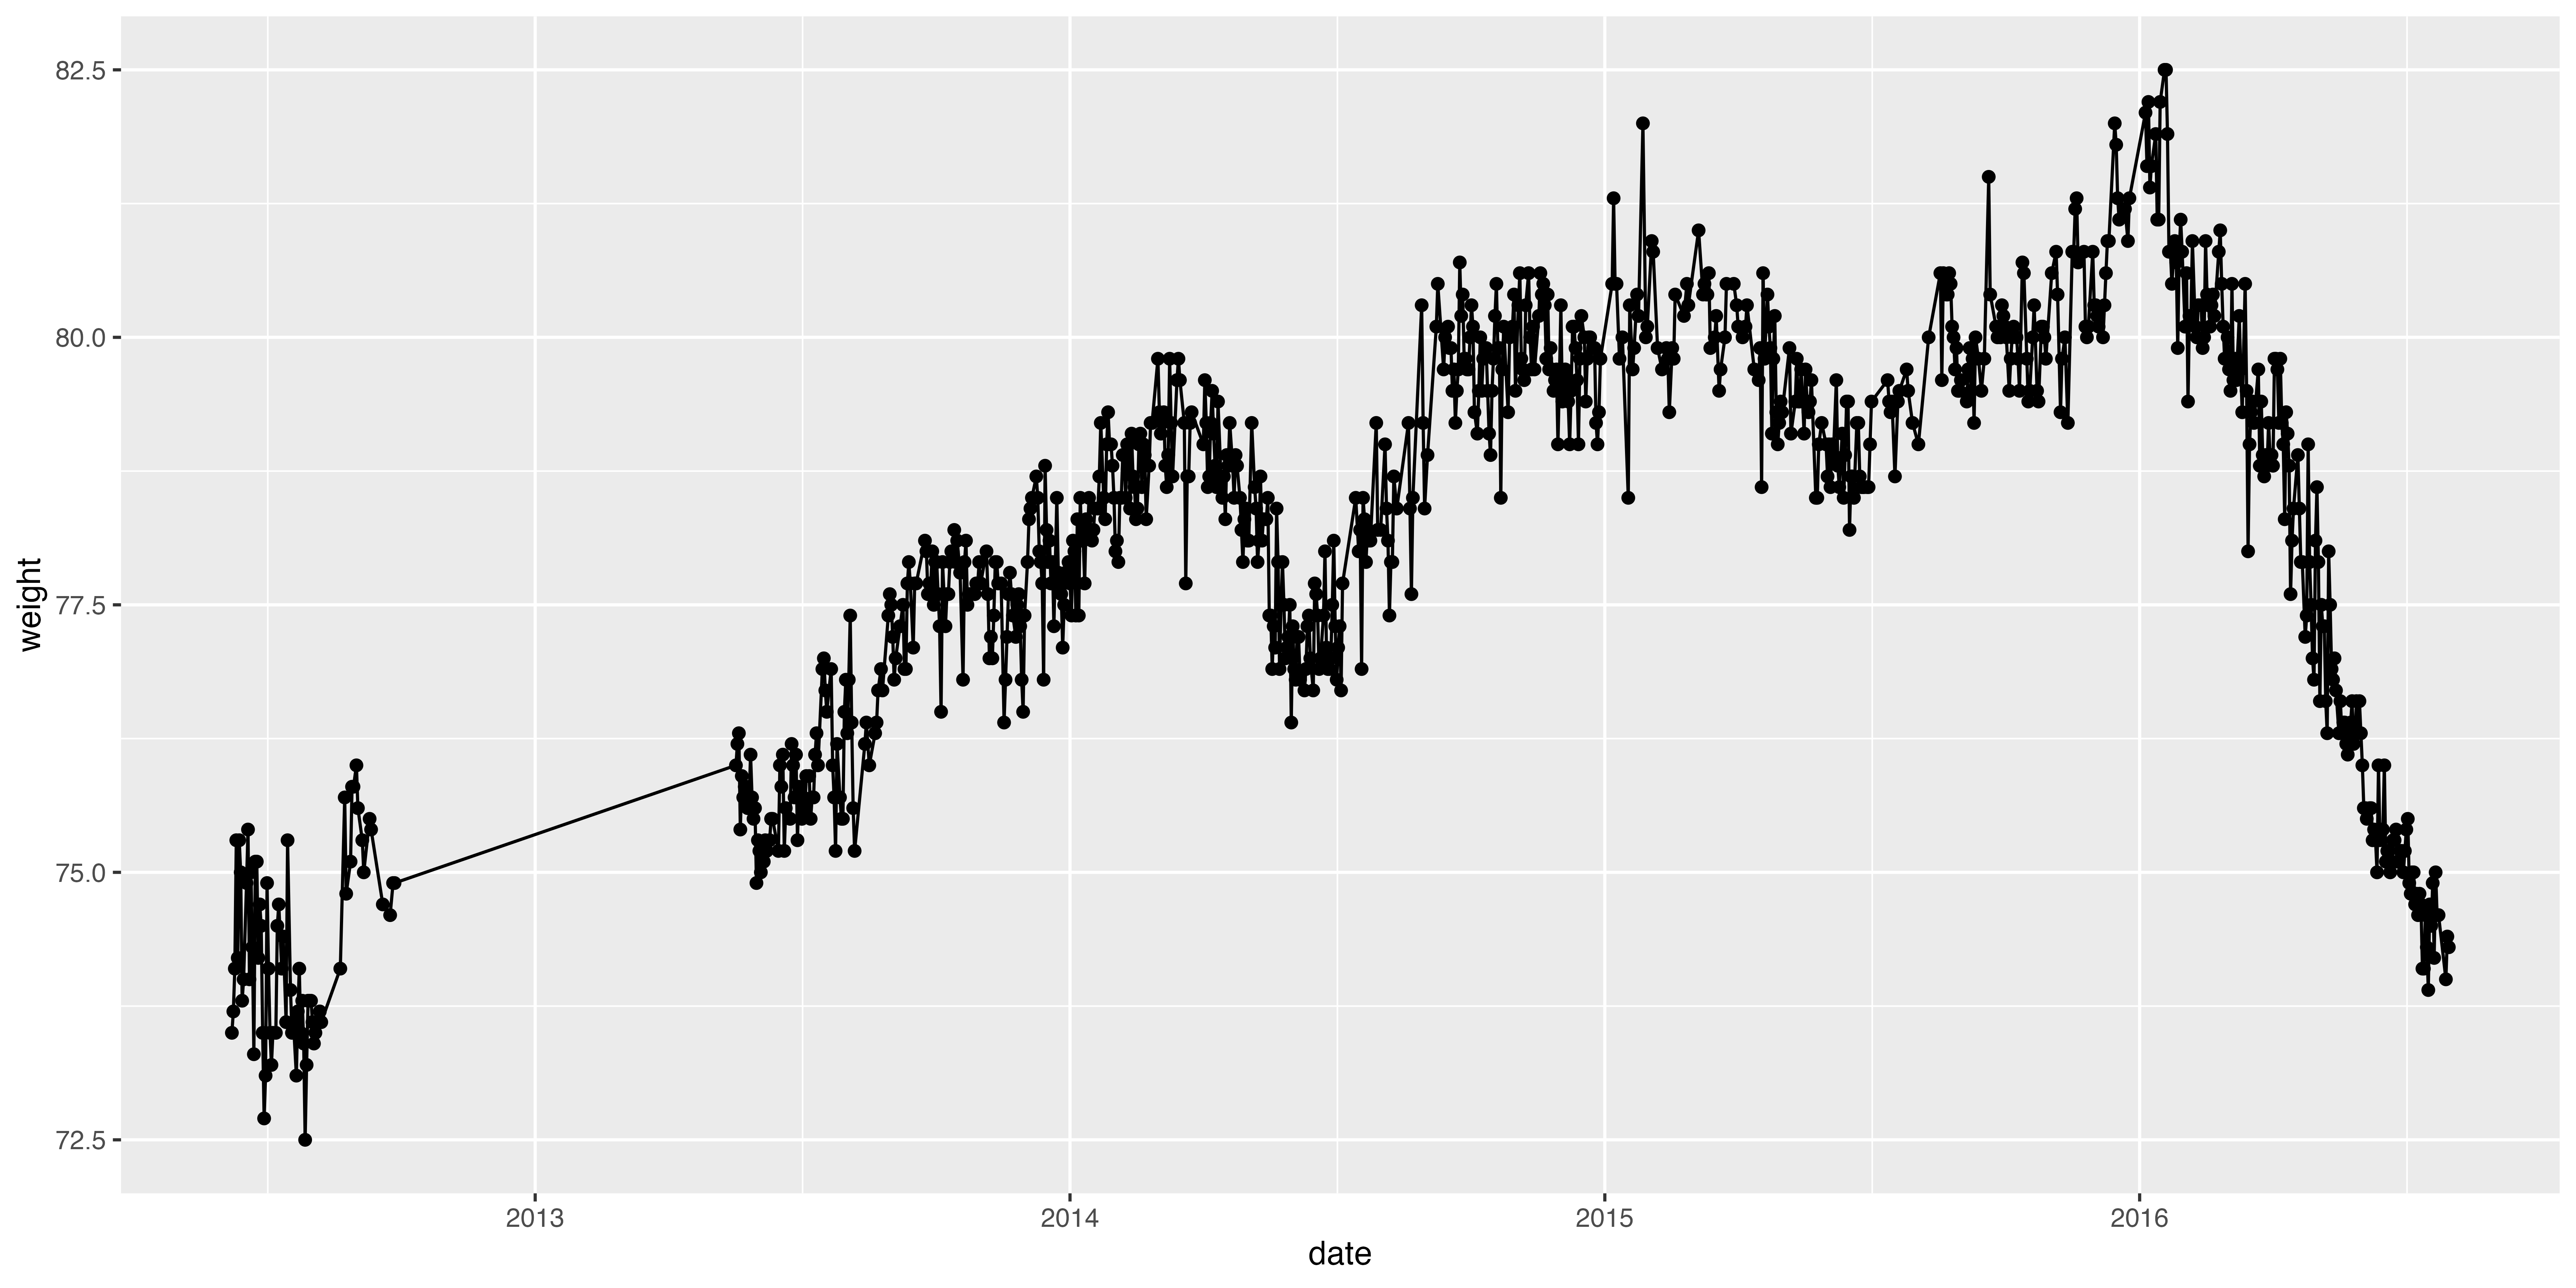
\includegraphics[keepaspectratio,width=12cm]{../images/02_Numbers/ggplot_sample_03.png}
	\caption{ggplot2による出力例3}
	\label{fig::03_08}
\end{figure}

図\ref{fig::03_06}には複数のプロット例を挙げました\footnote{この図の元になったデータは，2020年のプロ野球選手の身長や体重，年棒などをまとめたものです。ここでは身長，体重を守備位置やチームといった群の関係とともに表しています。}。一番上の段，左側にあるのは散布図です。X軸Y軸に変数があり，データがどのように散らばっているかを目で見ることができます。点を打つときは群ごとに色を変えてみました。最上段右図はボックスプロットと呼ばれる図です。4つの群の平均値とデータの散らばりが図示されています。真ん中の段の左図はボックスプロットと同じ情報ですが，ボックスプロットとは違う表現をしたものです。すなわちデータの散らばりを左右対称のヒストグラムのように描いたもので，わかりやすくするためにデータ点もその上にプロットしてみました。真ん中の段の右図はバープロット，棒グラフと呼ばれるもので，4つの群の平均値を高さで表しています。一番下の段にあるのはヒストグラムで，どの階級に何件のデータが入っているかを高さで表たものになっています。

図\ref{fig::03_07}に示したのは散布図ですが，群ごとに分けて表示してみました。またプロットするときの模様も，別のラベルごとに変えてみました。

図\ref{fig::03_08}に示したのは折れ線グラフです。これは私の体重変化の記録で，横軸が日付で縦軸が体重になっています。横軸に連続的な意味がある場合は各データ点がつながるように表現することで変化を表すことができます。

ここでは様々な図の表現の仕方がある，ということをわかってもらうことが目的であり，詳しいプログラムの書き方は第\ref{m03_introR}講でやりますので割愛します\footnote{気になる人は\citet{Kieran2018}や\citet{紀ノ定2021}を参照してください。またインターネット上には様々な資料が公開されているので，\texttt{ggplot2}で検索してみてください。}。強調したいのは，一枚の図の中にはラベルや色を変えることでいろいろな情報を埋め込むことができるということと，これらの図はいずれも描画言語による命令文の積み重ね=言葉で書かれている，ということです。コンピュータ言語という特殊な言葉ではありますが，どのように描くかということを指定するだけで，形状は機械がデータから作り上げるのです。このスクリプトを見ると誰でも同じ図を描くことができるので再現性が確保されていることを理解してください。

データ分析をするに当たってデータを図にするのですが，どのような図・色・形にすれば最もわかりやすく情報を表現できるか，ということを考えて図表のデザインをしなければなりません。図のデザイン(設計)は「図に書き込みたい情報は何かを考え，準備する」ところから始まり，縦軸・横軸で何を表すか，色・形・大きさで何を表現するか等を順に情報として追加していくことで行います。基本的には次のようなステップでデザインしていきます。
\begin{enumerate}
	\item X軸Y軸にどのような変数を置くかを考える。
	\item X軸Y軸から出来上がるキャンバスに，点や線，何をプロットするのかを指定する。
	\item その上にモデルを加えて，元のデータとの対応を考えたりする。別のデータを重ねることもある。
\end{enumerate}

ここでプロットと尺度水準のことを考えてみましょう。X軸もY軸も量的な変数であれば散布図でその変数の関係を表現できます。X軸が名義尺度水準でY軸が量的な変数であれば，散布図もX軸の対応する水準の上に並ぶような形になります。図\ref{fig::03_09}には2つの散布図の例がありますが，図の左は量的変数と量的変数のプロット，右は質的変数と量的変数のプロットになっています。このように同じ散布図であっても，変数の種類が違うと見え方が異なります。とくに右の図は散布図にするより，各水準の平均値を比較するようなバープロットのほうが情報を伝えやすいかもしれません。しかしいずれも散布図で，X軸が質的変数であるときは特殊なならびになるだけだ，という点はこの後の話と大きく関わってきますので，頭の片隅のどこかに置いておくようにしてください。
\begin{figure}[ht]
	\centering
	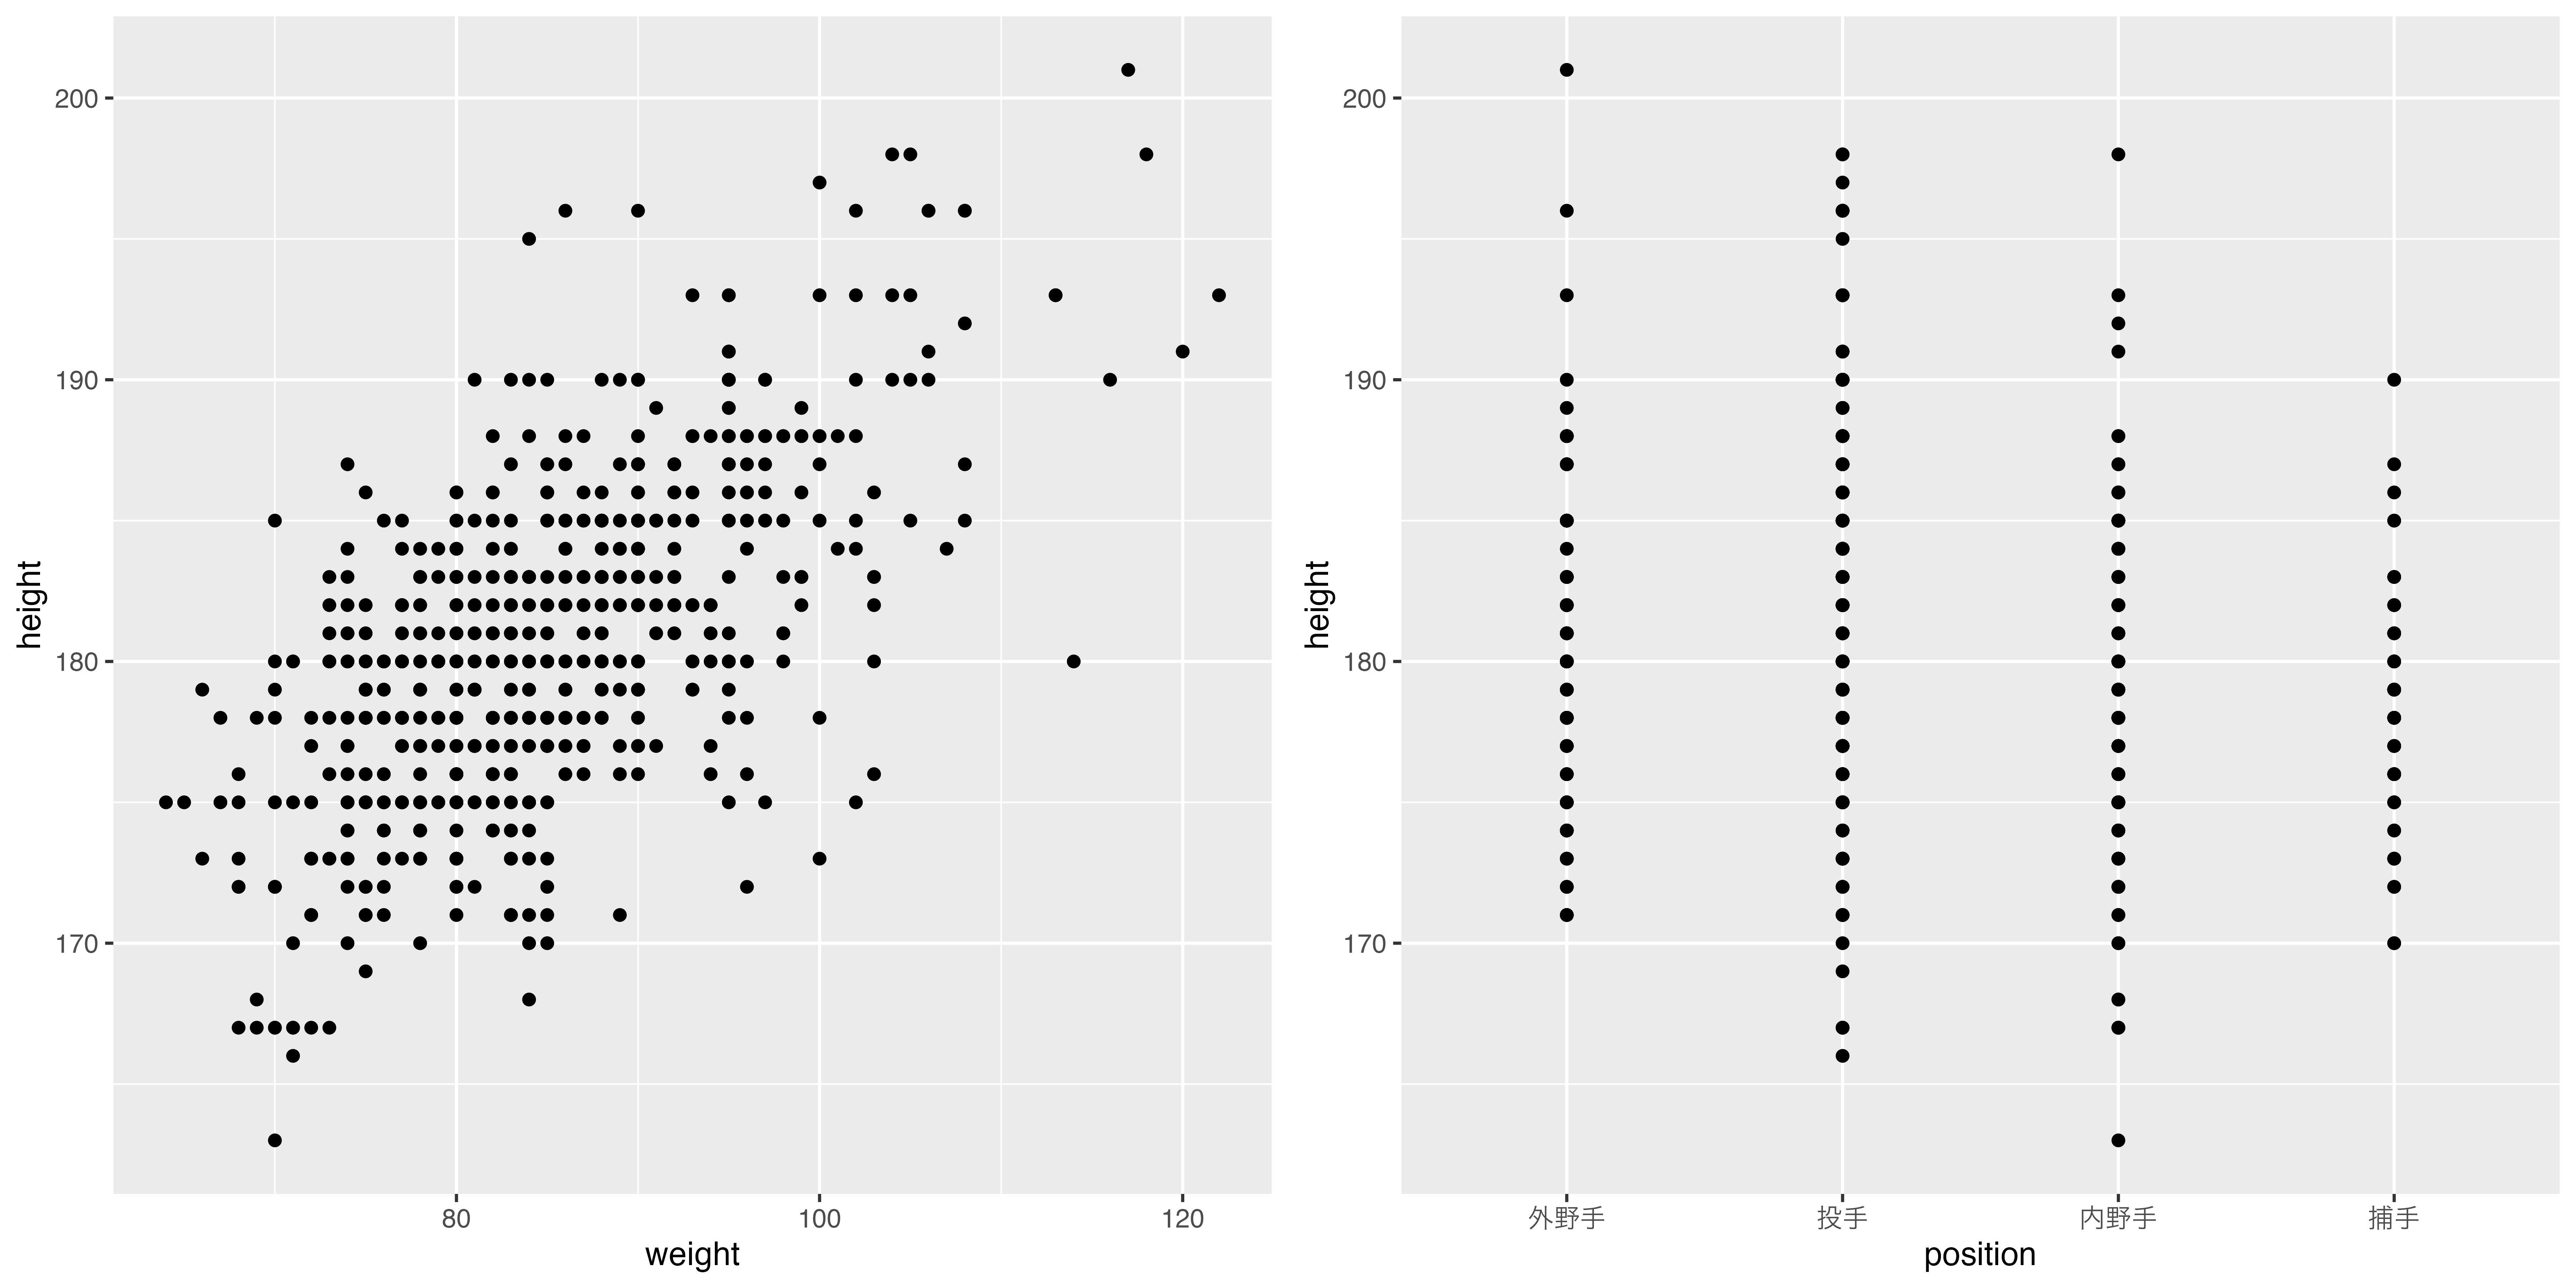
\includegraphics[keepaspectratio,width=12cm]{../images/02_Numbers/ggplot_sample_04.png}
	\caption{横軸と図の形}
	\label{fig::03_09}
\end{figure}

ところで，たかがグラフを描くためだけに，設計手順を書き下すなんて面倒なことを，と思うひともいるかもしれません。しかし描画の文法化の逆を考えればその利点が見えてきます。作図をこのように文法に沿って言葉で表現するようにしたことで，客観性の担保，再現性の確保にくわえ，どのデータをどのように表現したかったのかが明らかになるわけです。これの逆とはつまり，意図を隠し，主観的で再現できない情報を提示していることになります。これは科学的な態度と正反対です。残念ながら，世の中には悪意を持った人間による人為的で不合理な印象操作を目的とした図表が溢れています。データは可視化することでその特徴を把握しやすくするのですが，逆に視覚的特徴に引っ張られることで異なった印象を持たされることがあります。意図的に悪用すれば，議論をミスリードできます。統計的なデータというのはとくに嘘をついたり誤った印象を与えることがやりやすい領域であるが故に，とくにこの点については注意が必要なのです。

メディアリテラシーという観点からは，\citet{高木196807}など多くの良書があります。
一方，どうして図表をよみまちがえるのか，その知覚・認知的な観点からは\citet{Kieran2018}に詳しく書かれています。
\citet{Kieran2018}は上でもふれた\texttt{ggplot}の入門書なのですが，その1章はほとんど心理学です。
視覚のゲシュタルト性などを例に挙げながらどういう見え方，見せ方をしなければならないかについて丁寧に論じられているので，是非目を通してみてください。

\section{付録}

参考までに，図\ref{fig::03_05},\ref{fig::03_06},\ref{fig::03_07}を描写したコードを掲載しておきます。
Rによるコードの書き方や，これらの意味については第\ref{m04_usingR}講で行います。

なお，描画に使われているデータは，野球選手の身長や体重のデータ(コード内オブジェクト名は\texttt{sample})と，筆者の時系列的な体重変化のデータ(コード内オブジェクト名は\texttt{weight})であり，これらを読み込むコードは記載されていません。

\begin{lstlisting}[language=c++,label={code::03_01},caption={ggplot2による描画コード}]
# 散布図
g1 <- ggplot(sample, aes(x = height, y = weight, colour = team, fill = team)) +
  geom_point()

# ボックスプロット
g2 <- sample %>%
  select(position, height) %>%
  na.omit() %>%
  ggplot(aes(x = position, y = height, fill = position)) +
  geom_boxplot()

# バイオリンプロット
g3 <- sample %>%
  select(position, height) %>%
  na.omit() %>%
  ggplot(aes(x = position, y = height, fill = position)) +
  geom_violin(alpha = 0.7) +
  geom_jitter(alpha = 0.3)

# バープロット
g4 <- sample %>%
  select(height, position) %>%
  na.omit() %>%
  group_by(position) %>%
  summarise(mean = mean(height), sd = sd(height)) %>%
  ggplot(aes(x = position, y = mean, fill = position)) +
  geom_bar(stat = "identity", alpha = 0.7) +
  ylim(0, 200) +
  geom_errorbar(aes(ymin = mean - sd, ymax = mean + sd), width = .5)
  
# ヒストグラム
g5 <- sample %>% ggplot(aes(x = height)) +
  geom_histogram(binwidth = 1)

g6 <- ggplot(sample, aes(x = height, y = weight, 
            colour = team, fill = team, shape = position)) +
  geom_point() +
  xlab("height") +
  ylab("weight") +
  facet_wrap(~team)

# 折れ線グラフ
g7 <- weight %>% ggplot(aes(x = date, y = weight)) +
  geom_point() +
  geom_line()
\end{lstlisting}



\section{課題}
\paragraph{変数を見つける}次のような研究計画を立てた時に，変数として記録しておくべきなのは何でしょうか。
\begin{enumerate}
	\item 人の身長と体重の情報から，性別を予測することに興味がある。
	\item 人は寝ている間にたくさんの汗をかくという。一晩にかく平均的な寝汗の量に男女差があるのかどうかを調べたい。
	\item 結婚している人としていない人とで，幸福度に差があるかどうかを知りたい。
\end{enumerate}

\paragraph{尺度水準を理解する}次のそれぞれのデータは，どの尺度水準に該当するでしょうか。
\begin{enumerate}
	\item 個人を識別するために回答を求めた携帯電話番号の下4桁の数値
	\item 納税証明書に記載されている，個人の昨年度の納税額
	\item 年齢を直接質問するのがはばかられたため，「10代」「20代」「30代」「40代」「50代以上」の5段階について回答を求め，それぞれ1,2,3,4,5とコード化した数値
	\item 質問に対して「とてもそう思う」を5，「全くそう思わない」を1として，両者の間を均等に分割し2,3,4とする。また，「答えたくない」を0としてコード化した数値
	\item セルシウスさんが開発した，沸点を100，氷点を0として百分割した温度
	\item 温度とは分子の平均運動量であり，一定量の物質の温度をどんどん下げていくとこれ以上低くはならないという点が出てくる。そこを原点として作られた絶対温度K
	\item テレビ番組「帰れま10」では，ある外食チェーン店の豊富なメニューの中から，上位10品が何であるかを当てなければならない。このとき，それぞれのメニューに付される人気の順位を表した数字
\end{enumerate}

\end{document}
